\section{SpatialClaw}
\label{sec:method}

\ours{} realizes this code as the action interface through a persistent Python workspace for spatial reasoning.
Rather than exposing a larger menu of spatial tools, it lets the agent turn visual evidence into inspectable spatial analyses that can be composed and revised over multiple steps.
For each example, \ours{} creates a persistent Python kernel pre-loaded with the input frames and a set of primitives spanning perception modules (e.g., depth estimation, segmentation) and scientific libraries (e.g., NumPy~\citep{harris2020array}, SciPy~\citep{2020SciPy-NMeth}, Matplotlib~\citep{Hunter:2007}), and asks a VLM-backed agent to write one executable code cell at a time.
Each cell can create masks, reconstructions, plots, or numeric summaries, and the resulting program state remains available to later cells.
The next action is conditioned on text output, variable summaries, and rendered intermediate images from previous steps.
The remainder of this section formalizes these two components: the persistent kernel workspace that maintains shared program state across execution steps (\S\ref{sec:workspace}), and the outer agentic loop that coordinates planning, code generation, feedback assembly, and answer submission (\S\ref{sec:loop}).

\begin{figure}[t]
    \centering
    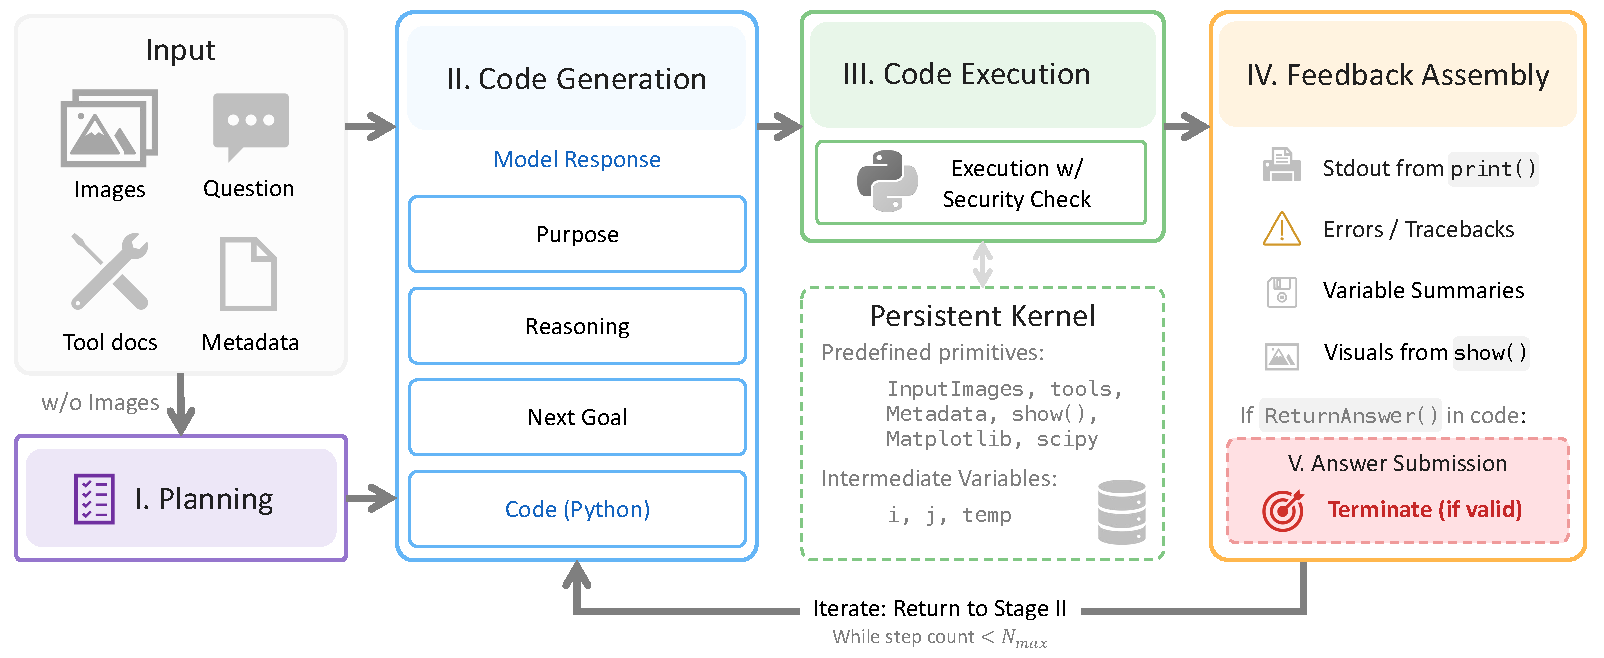
\includegraphics[width=\linewidth]{figures/pdf/method_loop.pdf}
    \caption{\textbf{Agentic loop for iterative code execution.} 
    \ours{} wraps a persistent kernel in a five-stage loop. A planner receives the question and tool documentation but not the images, and produces an analysis plan. The main agent generates a Python cell executed in the persistent kernel. Feedback comprising stdout, variable summaries, and images registered via \texttt{show()} is appended to the model context. The loop continues until the agent submits an answer with \texttt{ReturnAnswer()} or the step count has reached the predefined maximum $N_{\text{max}}$.}
    \label{fig:method_loop}
\end{figure}


\subsection{Persistent Kernel Workspace}
\label{sec:workspace}

The workspace is initialized once for an example and discarded after the system terminates.
It keeps all intermediate results as ordinary Python variables, so any object produced during execution, including segmentation masks, depth maps, numeric arrays, and rendered plots, remains accessible to subsequent code cells.
As a result, the agent does not need to choose the complete analysis in advance.
It can start with a coarse computation, inspect the result, and refine the analysis against the observed evidence. The kernel exposes six public entry points.
\begin{enumerate}[leftmargin=2em, itemsep=1pt, topsep=1pt]
    \item \texttt{InputImages} contains the sampled frames or images.
    \item \texttt{Metadata} contains frame rate, duration, and frame indices for video inputs, enabling the agent to reason about temporal structure when questions reference specific timestamps.
    \item \texttt{tools} exposes evidence-producing perception and geometry primitives.
    \texttt{Reconstruct} wraps Depth Anything 3~\citep{depthanything3} and returns per-frame depth, camera intrinsics, camera extrinsics, and dense point maps.
    \texttt{SAM3}~\citep{carion2025sam} produces image or video masks from text, point, or box prompts.
    The \texttt{tools} module also includes lightweight utilities for mask operations, geometric computations, and visualizations.
    These utility functions simplify common operations such as mask manipulation and geometric computation, but the agent is not limited to what they provide; any operation can also be implemented directly over arrays or through the scientific libraries (\texttt{NumPy}, \texttt{SciPy}, \texttt{Matplotlib}) available in the execution environment. Full descriptions of all tools and utilities are provided in Appendix~\ref{app:tools}.
    \item \texttt{show(\ldots)} registers an image to be embedded directly into the agent's context at the next step, allowing the agent to visually inspect intermediate results such as masks, depth maps, or annotated frames before deciding what to do next. Figures rendered via \texttt{matplotlib} (\texttt{plt.show()}) are captured in the same manner and included in the agent's next observation.
    \item \texttt{vlm} dispatches queries to a separate VLM session, returning the response as plain text without embedding images into the main agent's context.
    \texttt{vlm.locate(\ldots)} performs visual grounding, returning bounding boxes.
    \texttt{vlm.ask\_with\_thinking(\ldots)} handles questions that fall outside the perception toolset, such as those requiring commonsense reasoning or artistic style recognition. 
    Further details on the prompts used for each VLM session are given in Appendix~\ref{app:prompts}.
    \item \texttt{ReturnAnswer(\ldots)} submits a candidate answer.
\end{enumerate}
Together, these entry points form a self-contained computational environment: the agent reads observations through \texttt{InputImages} and \texttt{Metadata}, builds up spatial evidence via \texttt{tools}, inspects intermediate results through \texttt{show(\ldots)}, queries a separate VLM session when needed via \texttt{vlm}, and commits a final answer through \texttt{ReturnAnswer(\ldots)}.
How the agent sequences these actions across multiple steps is governed by the outer loop described next.

\subsection{Spatial Reasoning Loop: Code, Inspect, and Revise}
\label{sec:loop}

The persistent kernel provides a runtime environment for the action interface, but does not by itself prescribe when to plan, when to act on the observed evidence, and when to commit to an answer.
We therefore wrap the kernel in a five-stage outer loop (Fig.~\ref{fig:method_loop}) covering planning, code generation, code execution, feedback assembly, and answer submission.
The loop follows standard agent control structures and serves as a stable scaffold under which the construct, inspect, and revise pattern operates consistently across examples.
The loop prescribes the order and termination conditions of each stage, but not how the agent should reason spatially within them; that reasoning discipline is encoded in the system prompt. Details of the agent system are provided in \S\ref{app:system}.

\paragrapht{Disciplined reasoning via system prompt.}
\ours{} imposes structure on the open-ended Python action space through a unified system prompt, without any benchmark-specific engineering.
The prompt defines both the runtime objects available in the kernel and the verification discipline the agent is required to follow.
The prompt encourages the agent to treat spatial conclusions as claims that should be cross-checked against multiple evidence sources where possible.
For instance, the agent is guided to resolve the relevant frame of reference, prefer metric computation over pixel-level impressions for geometric questions, and visually inspect tool outputs such as masks and annotated objects.
It is also encouraged to sanity-check numerical magnitudes and consider any apparent disagreements between visualizations and computed quantities before invoking \texttt{ReturnAnswer()}.
Because the prompt encodes general principles rather than few-shot examples or task-specific templates, the same configuration is applied across all benchmarks and backbone models without modification; more prompt details are given in \S\ref{app:prompts}.
With this discipline in place, the loop proceeds through five stages as follows:

\paragrapht{Stage I: Planning.}
The planner runs in a separate LLM session, isolated from the main agent's execution context, with its own dedicated system prompt, and is invoked once per sample prior to execution.
Unlike the main agent's prompt, which focuses on general spatial reasoning discipline, the planner's prompt forbids executable code and pre-conclusion phrases, and instead instructs the planner to outline the analysis steps and the evidence to be acquired.
It receives the question, metadata, and tool documentation, but not the input frames for efficiency.
The resulting plan is appended to the main agent's system prompt before execution begins, providing the agent with a structured plan to follow.


\paragrapht{Stage II: Code generation.}
The main VLM-backed agent receives the question, the plan, the execution trajectory, and any images shown in previous steps.
At each step, it produces a structured response comprising \textit{purpose}, \textit{reasoning}, \textit{next goal}, and \textit{code} fields, formatted in markdown.
The \textit{code} field is a Python cell that implements the next analysis action, which can call perception primitives, transform their outputs, render intermediate evidence, or submit an answer via \texttt{ReturnAnswer()}.

\paragrapht{Stage III: Code execution.}
Before execution, a static checker parses the code's abstract syntax tree (AST) to reject disallowed modules and unsafe builtins without running the code; on failure, the framework injects a concise traceback into the context and prompts the agent to revise the code.
The validated cell is then executed in the persistent kernel.

\paragrapht{Stage IV: Feedback assembly.}
The next model context receives the standard output produced by the executed cell (e.g., values printed via \texttt{print()}), concise tracebacks for any failed execution, summaries of newly created variables including their type, length, and size, and any images registered through \texttt{show()} for visual inspection.
Because the kernel persists, later code can reuse earlier masks, reconstructions, plots, and partial analyses without recomputing them.
The agent can therefore revise the analysis after seeing a wrong mask, an implausible trajectory, or a depth distribution that does not support the intended comparison. 
This feedback is appended to the model context, making intermediate results accessible at any subsequent step.
The loop then returns to Stage II unless the agent has submitted an answer or the step count has reached the predefined maximum $N_{\text{max}}$.

\paragrapht{Stage V: Answer submission.}
When the agent determines that it has collected sufficient evidence, it submits an answer with \texttt{ReturnAnswer()}.
The loop terminates once the submitted answer conforms to the expected format for the question type (e.g., multiple choice, numerical, or free-form text). Otherwise, the loop continues to the next step. 
